\subsection{Velocity-rescaling thermostat}

\begin{figure}[H]
    \centering
    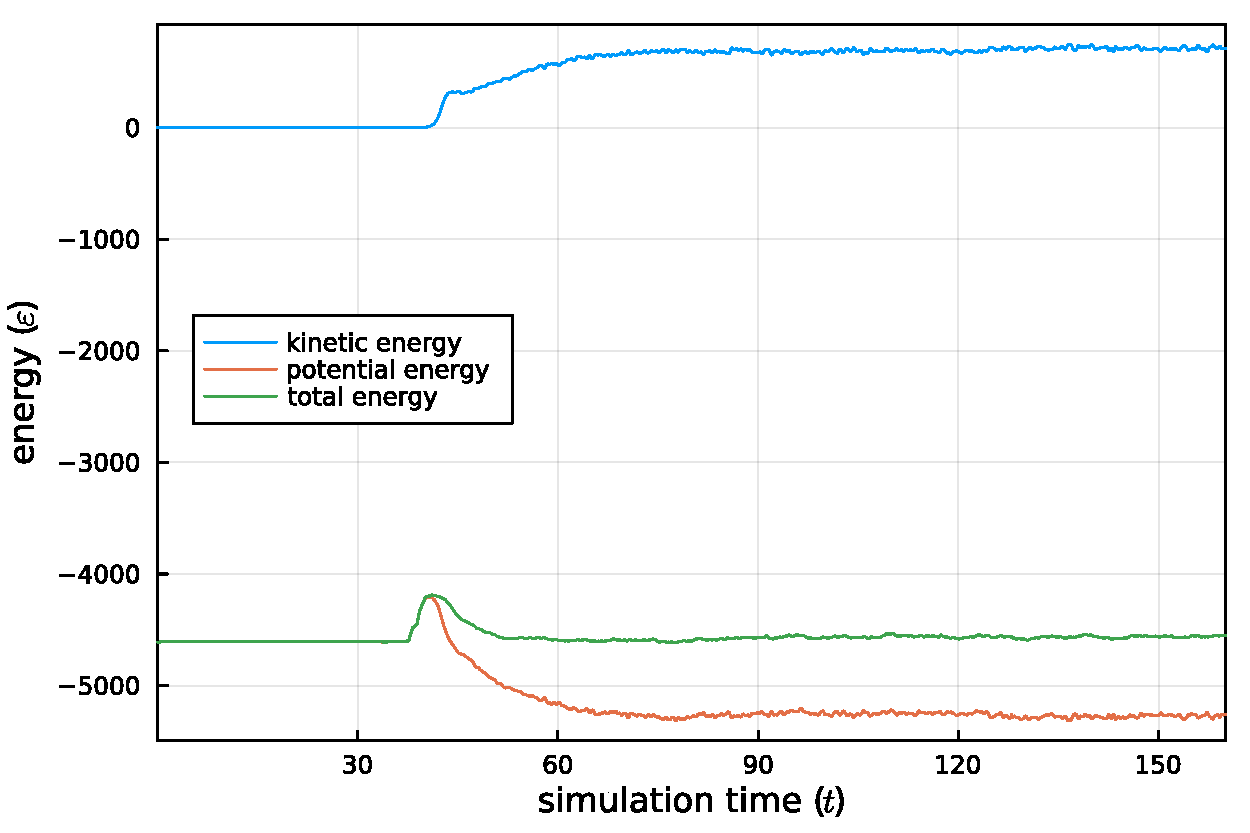
\includegraphics[width=0.8\textwidth]{e-t-no-thermostat}
    \caption{The dimensionless kinetic energy, potential energy, and total energy
        as a function of simulation time \(t\).}
    \label{fig:md5000}
\end{figure}

Now let us perform the molecular dynamics simulation.
First, we need to define our system. We select a system of \(1000\) particles,
with number density \(\rho = 0.75\), as in Vertlet\cite{Verlet}'s paper.
According to~\eqref{eq:L}, the box's side length will be about \(11.006 \sigma\).
We also need to set the initial positions and velocities of the particles.
We choose all the particles spaced by a constant distance, larger than \(1\)
to avoid the initial potential energy being too large (see~\eqref{eq:uljunit}),
in each direction, and all velocities to be zero.
We will first run \(5000\) MD steps to see the trend of the potential energy
and kinetic energy.
The corresponding code is in Snippet~\ref{lst:md5000}.

\begin{algorithm}[H]
    \caption{Running \(5000\) MD steps.}
    \label{lst:md5000}
    \begin{juliacode}
        particles = [Particle(rand(3), rand(3)) for _ in 1:1000]  # Generate 1000 particles
        box = CubicBox(length(particles), 0.75)  # Put them in a cubic box to s.t. number density = 0.75
        init!(particles, box, Even(), Uniform(zeros(Velocity)))  # Set the initial positions and velocities
        logger = Logger(length(particles))  # Start a logger tracking the MD steps
        Δt = 0.032  # The length of each time step
        take_n_steps!(logger, particles, box, 5000, Δt, VelocityVerlet())  # Run MD simulation
    \end{juliacode}
\end{algorithm}

After the code finishes, we plot the dimensionless kinetic energy, potential energy,
and total energy as a function of simulation time \(t\) in Figure~\ref{fig:md5000}.
After \(5000\) steps, which is around \(160\) units of dimensionless time and
\qty{5e-11}{\second} in real world time, we seem to already reach thermal equilibrium.
As the figure shows, after \(t = 40\) we can see a substatial decrease in the potential energy
and increase in the kinetic energy, while the total energy keeps almost the same for
the whole time, as it should be.

To make sure the kinetic energy calculated using~\eqref{eq:kinetic} is correct, we compare
the difference between the last and the first steps of both the kinetic and potential
energies, \(T_\text{last} - T_\text{initial} \approx 707.97\) and
\(U_\text{last} - U_\text{initial} \approx -650.61\), so they are at the same magnitude,
the difference could come from the steady energy drifts caused by accumulation of
numerical errors.

The temperature is represented by Equation~\eqref{eq:T}:
%
\begin{equation}\label{eq:T}
    T = \frac{16\varepsilon}{N k_B} \sum_{i=1}^{N} \lvert \bm{v}'_i \rvert^2,
\end{equation}
%
where \(N\) denotes the number of particles, and \(\bm{v}_i\) represents the reduced
velocity of the \(i\)-th particle. The question arises: what does the value \(1.069\)
represent in terms of real-world temperature? Given that \(\varepsilon \approx 119.8 k_B\),
we have
%
\begin{equation}\label{eq:1069}
    1.069 = \frac{16 \times 119.8}{864} \sum_{i=1}^{864} \lvert \bm{v}'_i \rvert^2,
\end{equation}
%
leading to \(\sum_{i=1}^{864} \lvert \bm{v}'_i \rvert^2 \approx 0.48185\). Furthermore,
considering the relation
%
\begin{equation}
    v' = v \sqrt{\frac{m}{48\varepsilon}},
\end{equation}
%
and substituting this relation into Equation~\eqref{eq:1069}, we obtain
%
\begin{equation}
    \sum_{i=1}^{864} \lvert \bm{v}'_i \rvert^2 = \sum_{i=1}^{864} \lvert \bm{v}_i \rvert^2 \frac{m}{48\varepsilon} = 0.48185,
\end{equation}
%
which implies that
%
\begin{equation}
    \nicefrac{1}{2} m\sum_{i=1}^{864} \lvert \bm{v}_i \rvert^2 = 0.48185 \times 48\varepsilon / 2 \approx \qty{0.1193866}{\electronvolt},
\end{equation}
%
corresponding to approximately \qty{1385.42}{\kelvin}.

However, at \(t = 160\), the temperature is only around \(0.472\), far away from our desired
value: \(1.069\). So we need to add more kinetic energy to our system. How do we do that?
We should use what is called a \emph{thermostat}, which is
a modification of the basic molecular dynamics scheme with the purpose of maintaining the
temperature constant (on average).

\begin{algorithm}[H]
    \caption{Definition of the velocity-rescaling thermostat and its application
        on the velocities of the particles.}
    \label{lst:thermostat}
    \begin{juliacode}
        struct VelocityRescaling
            desired_temperature::Float64
        end

        function apply_coupling!(particles, thermostat::VelocityRescaling)
            t = temperature(particles)
            for particle in particles
                particle.velocity *= sqrt(thermostat.desired_temperature / t)
            end
            return particles
        end
    \end{juliacode}
\end{algorithm}

The simplest thermostat is a velocity-rescaling thermostat, as we can see, the equilibrium
temperature of our MD simulation after \(5000\) steps are not equal to our desired value.
So we can multiply the velocities of the particles by a factor \(\lambda\) to match our
desired temperature.
From Equation~\ref{eq:T}, we know that
%
\begin{equation}
    \lambda = \sqrt{\frac{ T_0 }{ T(t) }},
\end{equation}
%
where \(T_0\) is the desired temperature and \(T(t)\) is the current temperature as
calculated from the kinetic energy.
In this example, to match \(T_0 = 1.069\), \(\lambda = 1.505\).
And in Snippet~\ref{lst:thermostat}, we show the definition of our thermostat type
\code{VelocityRescaling} and rescaling function \code{apply_coupling!}.

\begin{figure}[H]
    \centering
    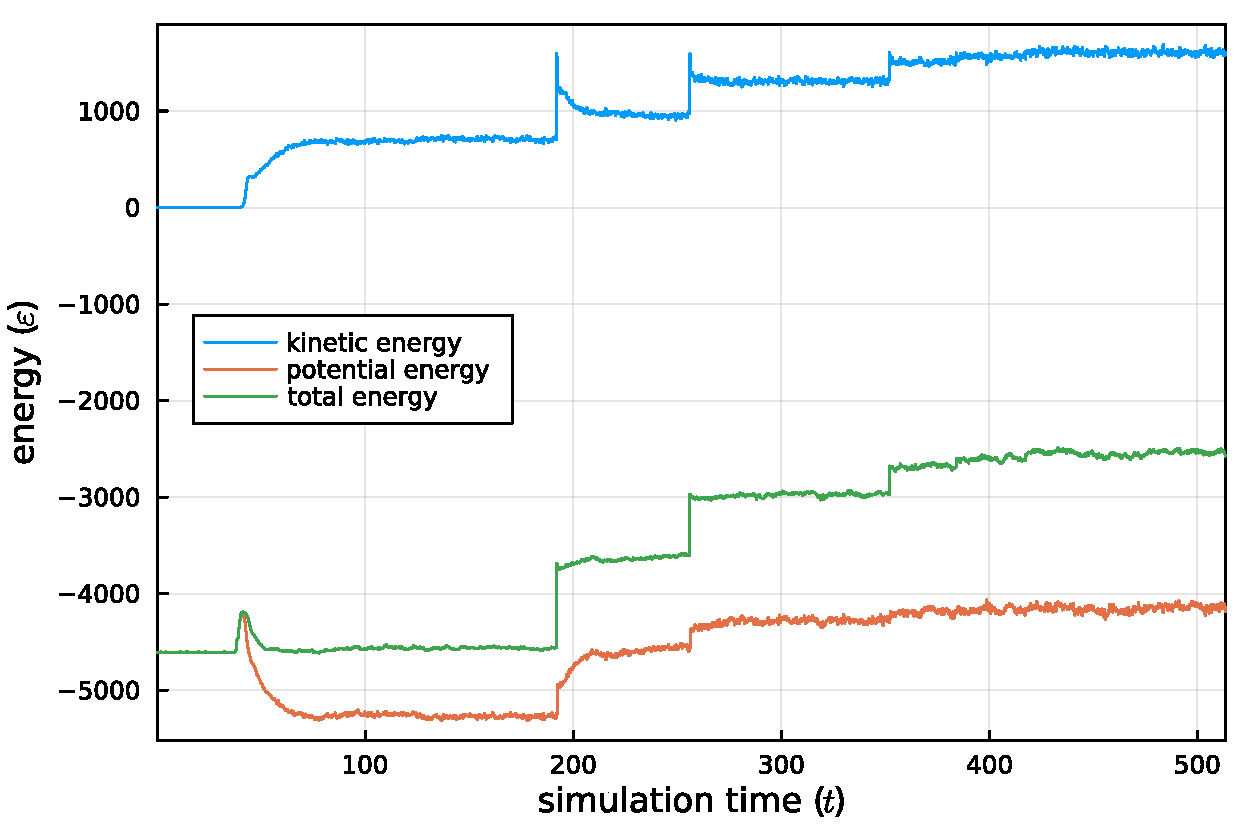
\includegraphics[width=0.8\textwidth]{e-t-thermostat}
    \caption{The dimensionless kinetic energy, potential energy, and total energy
        as a function of simulation time \(t\) after applying the velocity-rescaling
        thermostat for several times.}
    \label{fig:md-thermostat}
\end{figure}

One problem with this approach is that it does not
allow fluctuations in temperature which are present in the canonical ensemble.
There are better thermostats, e.g., the Berendsen thermostat.
Another problem is that we might not get the desired temperature even after we do the
rescaling one time since the system has changed and it has to restart thermalization
until equilibrium. Therefore, we may have to apply the thermostat consecutively
until the final desired value is reached.
In Figure~\ref{fig:md-thermostat}, we show the final results after several attempts.
After total \(16046\) steps, i.e., around \qty{1.60e-10}{\second}, the final temperature is
about \(1.073\).
We can see the final total energy is around \(-2575.04\), so starting from
\(E = U \approx -4610.29\) is a bit too low, that is why we are scaling up the velocities.
The reason of such low starting energy is that we used evenly distributed particles
with their shortest distance still larger than \(1\). If we use a random distribution
as our starting point, the starting potential energy will become very large and
may cause the MD simulation slower to converge.
We can see from the figure that after the first two rescaling attempts, the potential
energy also increases a little, causing our scaled kinetic energy drops by about the
same amount. That is when these particles are rearranging their positions and
it is why we cannot achieve our final goal in one shot.

We also plot Figure~\ref{fig:T-t} to show the change of temperatures as a function
of the simulation time.

\begin{figure}
    \centering
    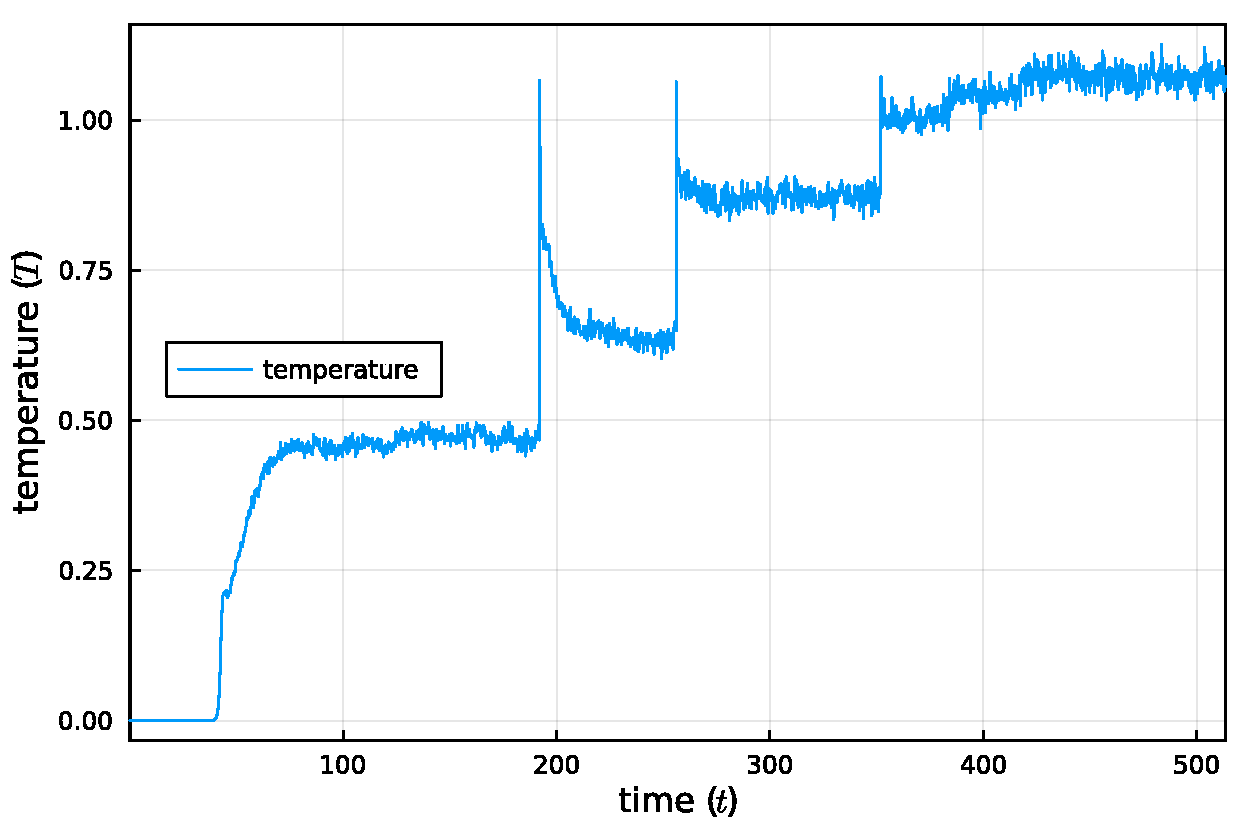
\includegraphics[width=0.8\textwidth]{T-t}
    \caption{The dimensionless temperature as a function of simulation time \(t\) after
        applying the velocity-rescaling thermostat for several times.}
    \label{fig:T-t}
\end{figure}
